\documentclass[conference]{IEEEtran}
\IEEEoverridecommandlockouts
% The preceding line is only needed to identify funding in the first footnote. If that is unneeded, please comment it out.
\usepackage{cite}
\usepackage{amsmath,amssymb,amsfonts}
\usepackage{cite}
\usepackage{algpseudocode}
\usepackage{graphicx}
\usepackage{textcomp}
\usepackage{xcolor}
\usepackage{amsthm}
\usepackage{algorithm}
%\usepackage{algorithmic}
\usepackage{epstopdf}
\usepackage{subfigure}
\usepackage{verbatim}


\newcommand{\tabincell}[2]{\begin{tabular}{@{}#1@{}}#2\end{tabular}}
\def\BibTeX{{\rm B\kern-.05em{\sc i\kern-.025em b}\kern-.08em
    T\kern-.1667em\lower.7ex\hbox{E}\kern-.125emX}}
\begin{document}

\title{HTS:Research on Task Scheduling Technology for Heterogeneous Storage\\
{\footnotesize \textsuperscript{*}Note: Sub-titles are not captured in Xplore and
should not be used}
\thanks{Identify applicable funding agency here. If none, delete this.}
}

\author{\IEEEauthorblockN{1\textsuperscript{st} Given Name Surname}
\IEEEauthorblockA{\textit{dept. name of organization (of Aff.)} \\
\textit{name of organization (of Aff.)}\\
City, Country \\
email address}
\and
\IEEEauthorblockN{2\textsuperscript{nd} Given Name Surname}
\IEEEauthorblockA{\textit{dept. name of organization (of Aff.)} \\
\textit{name of organization (of Aff.)}\\
City, Country \\
email address}
\and
\IEEEauthorblockN{3\textsuperscript{rd} Given Name Surname}
\IEEEauthorblockA{\textit{dept. name of organization (of Aff.)} \\
\textit{name of organization (of Aff.)}\\
City, Country \\
email address}
\and
\IEEEauthorblockN{4\textsuperscript{th} Given Name Surname}
\IEEEauthorblockA{\textit{dept. name of organization (of Aff.)} \\
\textit{name of organization (of Aff.)}\\
City, Country \\
email address}
\and
\IEEEauthorblockN{5\textsuperscript{th} Given Name Surname}
\IEEEauthorblockA{\textit{dept. name of organization (of Aff.)} \\
\textit{name of organization (of Aff.)}\\
City, Country \\
email address}
\and
\IEEEauthorblockN{6\textsuperscript{th} Given Name Surname}
\IEEEauthorblockA{\textit{dept. name of organization (of Aff.)} \\
\textit{name of organization (of Aff.)}\\
City, Country \\
email address}
}

\maketitle

\begin{abstract}
In order to meet different workload demand, a large number of heterogeneous storage devices are usually deployed on each node in the data center, i.e. SSD and HDD. However, data processing frameworks such as MapReduce often considers that hardware is homogeneous and task scheduling is not aware of the difference between storage devices. In this case, if a large number of tasks are scheduled to low-speed storage nodes, it will greatly cause data processing bottlenecks. In this paper, we formulate Heterogeneous Storage-aware Task Scheduling Problem(HTS), and show its NP-hardness. In order to solve this problem, a stochastic algorithm is proposed, whose distance from the optimum value is within t with high probability. Experiments show that the algorithm can improve the performance of Hadoop default scheduling mechanism by 40\%.
\end{abstract}

\begin{IEEEkeywords}
big data processing, heterogeneous storage, task scheduling
\end{IEEEkeywords}

\section{Introduction}

Nowadays, in data centers that support big data processing platforms i.e. Hadoop\cite{b14} and Spark\cite{b15}, there are more and more heterogeneous devices. On the one hand, due to the purchase of hardware devices from different hardware providers, such as Dell\cite{b16} and Samsung\cite{b17}, the different standard hardware  lead to heterogeneous; on the other hand, the use and maintenance of equipment may also lead to heterogeneous. However, the underlying heterogeneity of devices is often neglected in big data platforms, which results in the mismatch between upper software and lower hardware. The result is a waste of hardware resources or low performance of big data processing.

In order to improve the performance of big data processing, we focus on heterogeneous storage devices. A data processing workload, named a job, are usually divided into parallel tasks and scheduled to each node for execution. A task execution is usually divided into two parts, the first part is the data reading stage, and the other part is the task execution stage. Experiments show that if the a task read data from low-speed storage devices, the data read stage will be the bottleneck of task execution. Therefore, what we need to do is to select high-speed and low-load disks(If there are a large amount of tasks reading data on a high-speed disk at the same time, it may also cause bottlenecks in task execution.) for tasks as much as possible.

Most of the previous work focused on data locality\cite{b18}, deploying tasks close to data, but ignore the performance of storage devices. Although some work \cite{b1}\cite{b6}\cite{b7} considers heterogeneous storage devices, they didn't specify the performance of storage devices. HDFS\cite{b19}makes a clear distinction between SSD and HDD, and tasks are scheduled according to it. In fact, there are a large number of heterogeneous storage devices in the data center, and it is one-sided to devide the storage devices into two categories.

In this paper, we focus on the data reading stage in the execution of tasks. There are two aspects that affect data reading in task execution, one is the read performance of the disk itself, the other is the load of the disk, that is, the number of tasks that are reading the data from the disk. Then, it is described as an optimization problem, and we propose greedy algorithm and stochastic algorithm to solve the problem. Experiments show that the performance of the proposed algorithm is 40\% better than that of the default algorithm such as hadoop. More concretely, our contributions are as follows: 
\begin{itemize}
\item We present a motivational study to demonstrate the necessity of sloving the problem by investigating impact of reading data during the task execution phase.
\item We propose heterogeneous storage-aware task scheduling problem,  which is formally described and proved to be NP-hard. Then we propose  heuristic algorithm, named HTS-greedy, and  a performance-guaranteed
random algorithm, called HTS-rdm, to solve this problem. The solution found by the HTS-rdm algorithm can approach the optimal solution with probability  1 - O($e^{-t^2}$) where $t$ denotes the 
the difference between solution found by the HTS-rdm and the optimal solution.
\item We implemente the above algorithm through simulation experiments. The experimental results show that the performance of the proposed algorithm is improved by 40\% compared with the default data reading mechanism in hadoop.
\end{itemize}

The rest of the paper is organized as follows. The related works are presented in Section \ref{RELATED_WORKS}. In Section \ref{RELATED_WORKS}, we present the related works of the HTS problem. Then we propose our system model and our algorithm in Section  \ref{SYSTEM_MODEL} and Section  \ref{DESIGN_ALGORITHM}. At last, we conclude this paper in Section \ref{CONCLUSION} by summarizing our main contributions.
\section{RELATED WORKS}\label{RELATED_WORKS}
The related works consist of two aspects. On the one hand, due to limited link bandwidth, some work is focused on data locality. On the other hand, in heterogeneous environments, it is not enough to consider data locality alone and some other studies have been carried out to accelerate data processing by studying hardware heterogeneity \cite{b1}.

Due to the limited network bandwidth resources in data center, if a large amount of data is transmitted between nodes during task execution, it will greatly affect the task performance. Therefore, processing data locally as much as possible can improve performance, i.e. placeing map task to the node which stores the input data. Matei et al. \cite{b2} proposes delay scheduling to assure data locality. Delay scheduling considers that when a node has idle slots, priority should be given to scheduling tasks with input data at that node, and delayed scheduling tasks without input data at that nodes. Ganesh \cite{b3} makes multiple replicas of high-frequency data by analyzing the access frequency of data, improve the data locality in this way. Cristina \cite{b4} proposes a distributed adaptive data replication algorithm DARE, which can help scheduler achieve better data locality. Jalaparti \cite{b5} believes that most of the production work is repetitive and predictable, which enables us to plan ahead. Coordinating and improving the tasks and data placement of these jobs can effectively reduce bandwidth usage and improve data locality. All of these work improves the performance of data processing by improving data locality.

However, in heterogeneous data centers, due to the different performance of data storage devices, task completion time is often different. At present, some of the existing work is based on the research of storage heterogeneity, which accelerates the method of large data processing. Xu et al. \cite{b6} considers the current usability of underlying hardware (CPU, memory, I/O), but does not consider the performance differences of different storage hardware. Pan et al. \cite{b7} takes into account the performance between different storage, but the problem can not be formally described. et al. Wang B \cite{b8} uses Markov model to describe the use of nodes in the cluster to deploy data reasonably. However, the scheduling problem of tasks is not considered, and the heterogeneity of different storage media is also not considered. These work does not accurately define the differences between storage hardwares, and choosing low-speed storage for a large amount of tasks can also lead to bottlenecks.

The difference between those tasks and ours are that our work clearly defines the difference in disk read speed and that deploying tasks according to different disk read speed to avoid bottlenecks.

\section{SYSTEM MODEL AND PROBLEM FORMULATION}\label{SYSTEM_MODEL}
In this section, we first introduce the background of large data processing based on heterogeneous storage and build the system model. After that, the task scheduling problem with heterogeneous storage awareness is formulated as a  minimization problem whose objective is to minimize the maximum disk read time.

\subsection{Background and motivation}\label{AA}

A large number of query jobs are running on large data processing platforms, which have the requirements of low response lantacy and high quality of service. During execution, jobs are subdivided into parallel tasks which scheduled to heterogeneous nodes. However, the general task scheduler i.e. FIFO scheduler is based on the fact that nodes are homogeneous, and the nodes with low computational power and high computational power will be deployed with the same amount of tasks. Tasks deployed by nodes with low computational power will have a longer execution time. The query job doesn't finish untill the completion of all tasks. Therefore, this kind of scheduling mechanism may cause the execution time of jobs to be too long to guarantee low query latency.

Task execution time is usually divided into two parts, one part is the lantacy of reading data from disk, the other part is the time of task execution in CPU. Experiments show that the reading time of low-speed disks can account for 70\% of the total task execution time, as shown in \ref{tab1}. Therefore, in order to ensure low latency of query jobs, data can be read from low $read-time$ disks. In the following section, we will use $read-time$ to represent the performance of a disk. This value is the time required to read a data replica from disk i.e. 0.2s. The smaller the value, the better the disk performance. When reading N data from the disk, the total time is $read-time$ * N. In data centers, data is deployed in multiple copies on disks with different reading speeds. When data centers generate a large number of tasks, we consider deploying tasks to minimize the maximum disk $read-time$s,  thereby speeding up data processing.%tasks on high-speed disks and fewer tasks on low-speed disks to minimize the overall task's disk reading time, thereby speeding up large data processing.

\begin{table}[htbp]
	\caption{Comparisons of read time and execution time}
	\begin{center}
		\begin{tabular}{|c|c|c|c|}
			\hline
			\multicolumn{2}{|c|}{\textbf{For 640MB data}} \\
			\hline
			\textbf{Reading time from HDD}& \textbf{Execution time (WordCount)}\\
			\hline
			3s & 1.5s  \\
			\hline
		\end{tabular}
		\label{tab1}
	\end{center}
\end{table}

As shown in Fig.\ref{fig1} there are four disks in the data center: DISK1, DISK2, DISK3 and DISK4. Each disk has different $read-time$, and $read-time$ of the four disks , $T$, are 0.3, 0.1, 0.2 and 0.2, respectively. The deployment of data replicas is shown in Fig.\ref{fig1}. When tasks are deployed, a general scheduler may place tasks such as scheduling1, and the execution time of the task is max \{$T_1 * N_1$, $T_2 * N_2$, $T_3 * N_3$,  $T_4 * N_4$, \} = max\{0.3*1, 0.1*1, 0.2*3, 0.2*1\}=0.3. Storage-aware task schedulers may place tasks as scheduling2, with a task execution time of at least 0.2. Obviously, the scheduling2 is optimum.

\begin{figure}[!t]
	\centering
	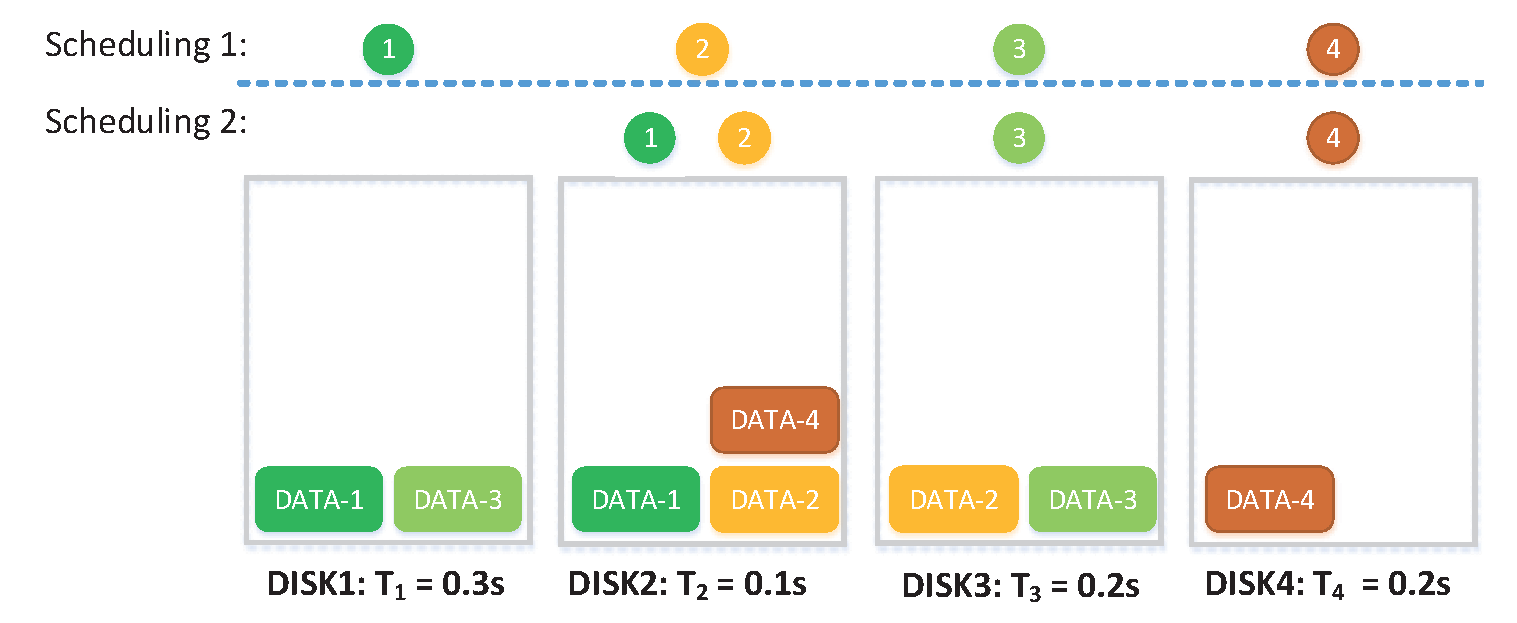
\includegraphics[height=1.4in]{fig1.eps}
	\caption{Comparison of task time between general task scheduling and disk-aware task scheduling. Scheduling1 is unaware of disk $read-time$ and the completion time of all tasks is max\{$T_1 * N_1$, $T_2 * N_2$, $T_3 * N_3$,  $T_4 * N_4$ \} = max\{0.3*1, 0.1*1, 0.2*3, 0.2*1\}= 0.3. Scheduling2 is aware of disk read time and the completion time of all tasks is max\{0, 0.1*2, 0.2*1, 0.2*1\} = 0.2. Scheduling2 is the optimum. }
	\label{fig1}
\end{figure}

Example shows that when choosing the disk of the input data for a task, two things need to be considered: the first is the $read-time$ of a disk, and the second is the amount of tasks that are taking the data from the disk as input, that is, the load of the disk. These two things are able to ensure that there are no bottlenecks in the process of reading data from disk and the data processing can be accelerated.

\begin{table}[!t]
	\Large
	\centering
	\footnotesize
	\renewcommand\arraystretch{1.2}
	\caption{NOTATIONS USED IN THIS PAPER.}
	\label{table-notations}
	\begin{tabular}{c|l}
		\hline
		$\mathbb{D}$ & \tabincell{l}{The set of heterogeneous disks in datacenter} \\
		\hline
		$\mathcal{M}$ & \tabincell{l}{The set of data in datacenter} \\
		\hline
		$\mathbb{T}$ & \tabincell{l}{The set of tasks to be scheduled} \\
		\hline
		$d_{i}$ & \tabincell{l}{The disk $i$ and $d_i \in \mathbb{D}$ } \\
		\hline
		$t_{j}$ & \tabincell{l}{The task $j$ and $t_j \in \mathbb{T}$ } \\
		\hline
		$m_{l}$ & \tabincell{l}{The data $l$ and $m_j \in \mathbb{M}$ } \\
		\hline
		$r_{l}^{k}$ & \tabincell{l}{The data replica $k$ of data  $m_l $ } \\
		\hline
		$read-time$ & \tabincell{l}{This time of reading a data block from disk } \\
		\hline
		$T_{i}$ & \tabincell{l}{The read-time of disk $d_i$} \\
		\hline	
		${I}_i^j$ & \tabincell{l}{A binary variable indicating if task $t_{i}$ choose the replica \\ that stored in $d_{i}$ as input  or not}\\
		\hline
		$\phi(t_j)$ & The data that task $t_j$ needs, and $\phi(t_j)$ $\in$  $\mathcal{M}$ \\
		\hline
		$\pi_{l}^{i}$ & \tabincell{l}{A binary variable indicating if data $m_l$ are \\stored at disk $d_i$ or not} \\
		\hline
		$h_{ul}$, $h_{dl}$ & \tabincell{l}{the channel fading coefficient for uplink and downlink} \\
		\hline
		$\phi(t_j)$ & The data that task $t_j$ needs \\
		\hline
		$N_(i)$ & Number of tasks which select data from disk i as input \\
		\hline
		$\tau$ & Size of each data replica in datacenter \\
		\hline
		$C$ & The number of replicas of each data. \\
		\hline
	\end{tabular}
\end{table}

\subsection{System Model}

The notations we need are shown in the table \ref{table-notations}. The data center is equipped with heterogeneous disks, and $\mathbb{D}$ is used to represent the set of all disks which are $d_{1}$, $d_{2}$, ...,$d_{|D|}$.  $\mathcal{M}$ denotes the set of all the data in data center, and each data is represented by $m_{1}$, $m_{2}$, ..., $m_{|M|}$. Each data $m_{l}$ has $C$ replicas which are $r_i^1$, $r_i^2$,... $r_i^{C}$ stored on $C$ different disks, with each data replica's size $\tau$, i.e. 64MB or 128MB. If the disk $d_{i}$ contains a replica of the data $m_l$, $\pi_l^{i}$ = 1. Otherwise, the $\pi_l^{i}$ = 0. In datacenter with heterogeneous disks, each disk has its own $read-time$ represented by $T_i$, and its value represents the time required to read a data replica from disk.

When the query job arrives, the job will be divided into parallel tasks. $\mathbb{T}$ denotes the set of all tasks which are $t_1$, $t_2$, ..., $t_{T}$. Each task $t_j$ corresponds to a unique input data $\phi(t_j)$. Since there are $C$ replicas of each data deployed in $C$ disks, the replicas of $\phi(t_j)$ exists in $C$ disks, assuming that it is $d_{j1}$, $d_{j2}$,... $d_{j|C|}$. So $t_j$ has $C$ choices.

Next, if the task $t_j$ chooses the replica sored in disk $d_i$, then $I_i^j$ = 1, where i belongs to \{$d_{j1}$, $d_{j2}$,... $d_{j|C|}$\}. In this case, the time of task $t_j$ reading the replica from disk $d_{j}$ is $I_i^j*T_i$. There may be some other tasks that select the other replicas in disk $d_{i}$, so the total $read-time$ of disk $d_{i}$ is $\sum_{j}I_i^j*T_i$. In order to avoid a large number of tasks to choose the same disk, resulting in data processing bottlenecks. Our objective is to minimize the maximum disk $read-time$.

\subsection{Heterogeneous Storage-aware Task Scheduling Problem Formulation ($\rm{HTS}$)} \label{HTS}

%$\mathcal{AP} \mathbb{AP}$ (~/~)

There are a large number of heterogeneous disks in the data center. If the scheduler are unaware of the heterogeneity of disks, it is likely that there are a large number of tasks that read data from the same low-speed disk, resulting in bottlenecks. To avoid this situation, we propose heterogeneous storage-aware task scheduling(HTS), as shown below. The optimization goal is to minimize the maximum disk $read-time$. Finally, by determining the value of the decision variable $I_i^j$, the appropriate disk is selected for each tasks to read the corresponding data. Detailed description is as follows:
\begin{align}
Min:&\;\;\;\;\;\max\limits_{i}\{\sum_{j}I_i^j*T_i\}\;[\rm{HTS}]\nonumber\\
s.t. 
&\;\;\;\;\;\sum_{i}I_i^j = 1,\;for\;\forall j\label{task-cons}\\
&\;\;\;\;\;I_i^j \leq \pi_{\phi(t_j)}^{d_i},\;for\;\forall i,j\label{data-cons}\\
&\;\;\;\;\;I_i^j\in\{0,1\},\;for\;\forall i,j\label{def-cons}
\end{align}

Constraint 1 indicates that task $t_j$ can only read its input data from one of all disks. Since one data is only stored on C disks, not all disks contain that data. Constraint 2 indicates task $t_j$ can only read its input data from the disks which stores its input data. $\phi(t_j)$ denotes task $t_j$'s input data and $\phi(t_j)$ = $m_j$. If one replica of data $m_j$ is stored in disk $d_i$, $\pi_{\phi(t_j)}^{d_i}$ = 1, otherwise $\pi_{\phi(t_j)}^{d_i}$ = 0. Constraint 3 denotes the range of decision variables, which can only be 0 or 1. $I_i^j$ = 1 indicates that task $t_j$ selects the replica stored on disk $d_i$ as input, while task $t_j$ = 0 is on the contrary.

The key to solve HTS problem is to determine the value of decision variables {$I_i^j$}. Next, we analyze the hardness of this problem and prove that the HTS problem is NP-hard. This is because the HTS problem can be reduced from the integer linear programming (ILP) problem, and the ILP problem is NP-hard, so HTS problem is NP-hard. The specific proof process is as follows.

\emph{Theorem 1:} The HTS problem is NP-hard.

\emph{Proof:}
The canonical form \cite{b11} of ILP is described below.

For $m\times n$ matrix \textbf{A}
\begin{align}
Min:&\;\;\;\;\;\textbf{c}^T\textbf{x}\;\;[\rm{ILP}]\label{ILP}\\
s.t. 
&\;\;\;\;\;\textbf{A}\textbf{x}\geq \textbf{b}\nonumber\\
&\;\;\;\;\;\textbf{x} \geq0,\nonumber\\ 
and
&\;\;\;\;\;\textbf{x} \in \mathbb{Z}^n\nonumber
\end{align}

Taking the special case of HTS problem, the parameters are set as follows:
\begin{itemize}
	\item $\mathbb{D}$ = \{$d_0$, $d_1$, $d_2$\};$T_0$ = 1, $T_1$ = 1, $T_2$=1; $\mathbb{M}$ = \{$m_0$, $m_1$, ..., $m_{n-1}$\}; $C$ = 3
	\item $T$ = \{$t_0$, $t_1$, ..., $t_{n-1}$\}
\end{itemize}

It means that there are 3 disks, $d_0$, $d_1$, $d_2$, in the data center, each disk with a $read-time$ of 1. A total of n data, and each data has three replicas which deployed in the three disks, respectively. When the query job arrives, the job is divided into n tasks, $t_0$, $t_1$, ..., $t_n$ to read n data,$m_0$, $m_1$, ..., $m_n$, respectively.

For this particular case, the problem description can be modified to:

\begin{align}
Min:&\;\;\;\;\;\max\{\sum_{j}I_0^j, \sum_{j}I_1^j, \sum_{j}I_2^j\}\;[\rm{HTS-sp}]\\
s.t. 
&\;\;\;\;\;I_0^j + I_1^j +I_2^j= 1,\;for\;\forall j\nonumber\\
&\;\;\;\;\;I_0^j, I_1^j, I_2^j\in\{0,1\},\;for\;\forall j \in[0,n)\nonumber
\end{align}

Let  $x$ = $\sum_{j}I_0^j$, $y$ = $\sum_{j}I_1^j$, $z$ = $\sum_{j}I_2^j$, and the problem description can be modified to:
\begin{align}
Min:&\;\;\;\;\;\max\{x,y,z\}\;[\rm{HTS-sp}]\\
s.t. 
&\;\;\;\;\;x + y + z = n\;\label{enlarge-cons}\\
&\;\;\;\;\;0 \leq x \leq n, x\in\mathbb{Z}\nonumber\\
&\;\;\;\;\;0 \leq y \leq n, y\in\mathbb{Z}\nonumber\\
&\;\;\;\;\;0 \leq z \leq n, z\in\mathbb{Z}\nonumber
\end{align}
In the minimization problem, x + y + z = n can be modified to x + y + z = n and let $R$ denotes $\max\{x,y,z\}$. 

Finally, HTS-sp problem is converted to:
\begin{align}
Min:&\;\;\;\;\;\max\{R\}\;[\rm{HTS-ILP}]\label{HTS-ILP}\\
s.t. 
&\;\;\;\;\;x + y + z \geq n\;\nonumber\\
&\;\;\;\;\;-x + R \geq 0 \nonumber\\
&\;\;\;\;\;-y + R \geq 0  \nonumber\\
&\;\;\;\;\;-z + R \geq 0 \nonumber\\
&\;\;\;\;\;0 \leq x \leq n, x\in\mathbb{Z}\nonumber\\
&\;\;\;\;\;0 \leq y \leq n, y\in\mathbb{Z}\nonumber\\
&\;\;\;\;\;0 \leq z \leq n, z\in\mathbb{Z}\nonumber\\
&\;\;\;\;\;R \geq 0, R\in\mathbb{Z}\nonumber
\end{align}

The decision version of 0-1 ILP (A variation in which only the restrictions must be satisfied, without optimization) is one of Karp's 21 NP-complete problems  \cite{b9}, so ILP is NP-hard. Further, the problem HTS-ILP in \ref{HTS-ILP} is an instance of ILP in\ref{ILP}, so the HTS-ILP problem is NP-hard.

On the one hand, when the optimal solution of HTS-ILP problem is obtained, the corresponding {x, y, z} can be converted into variable {$I_i^j$} in polynomial time by setting the value in \{$I_0^0$, $I_0^1$, ...,$I_0^{x-1}$, $I_1^{x}$, $I_1^{x+1}$, ..., $I_1^{x+y-1}$, $I_2^{x+y}$, $I_1^{x+y+1}$, ..., $I_2^{x+y+z-1}$\} to be 1, which will make the corresponding HTS-sp problem obtain the optimal solution. On the other hand, when the variable \{$I_i^j$\} make the HTS-sp problem obtain the optimal solution, the HTS-ILP also obtains the optimal solution by setting $x$ = $\sum_{j}I_0^j$, $y$ = $\sum_{j}I_1^j$, $z$ = $\sum_{j}I_2^j$. It can be seen from the above that any solution can be polynomially transformed between the HTS-sp and HTS-ILP. Therefore, HTS-sp is NP-hard. 

As a result of that HTS-sp is a special case in HTS, HTS problem is NP-hard.\hfill $\qedsymbol$

\section{DESIGN of ALGORITHMS FOR HTS PROBLEM}\label{DESIGN_ALGORITHM}

Due to the hardness of HTS problem, the optimal solution can not be obtained in polynomial time. In order to solve NP-hard problem, heuristic algorithm is the basic solution. At first, we propose a heuristic algorithm based on greedy idea, HTS-greedy. However, this kind of algorithm usually has no guarantee of quality, although in some cases it can get relatively good results, in some cases it can not. Considering further, we design a quality assurance algorithm HTS-rdm, which makes the feasible solution approximate to the optimal solution with a high probability.


\subsection{Heuristic Alogrithm}\label{Heuristic}

In this section, we propose a heuristic algorithm HTS-greedy. Using the greedy idea, the algorithm chooses the disk which stores $\phi(t_j)$ for each task $t_j$ and which has the minimum total $read-time$, and finally outputs one disk for each task.


%Alogoritm1
\begin{algorithm}
	%\renewcommand{\thealgorithm}{}
	
	\textbf{Require:} For each task $t_j$, decide a disk $d_i$ that stores one replica of data $\phi(t_j)$.

	\begin{algorithmic}[1]
		\For{each disk $d_i$} \label{HTS-greedy:init}
			\State $load_{i}$ $\gets$ 0
		\EndFor
		\State Result $\gets$ \{\}
		\For{each task $t_j$} 
			\State $d_{j1}$, $d_{j2}$,... $d_{j|C|}$ = f($\phi(t_j)$)
		
			$//$Function f is a mapping from data to disks that stores each replica of the data.
			\State $load_{j_{min}}$ $\gets$ $\min\limits_{l}$($load_{j_l}$)
			
			$load_{j_{min}}$ $\gets$ $load_{j_{min}}$ + $T_{j_{min}}$
			\State Result $\gets$ Result $\cup$
			\{$\left \langle t_j, d_{j_{min}}\right \rangle$\}
		\EndFor
	
	\State \textbf{Return} Result
	\end{algorithmic}
	\caption{HTS-greedy}\label{HTS-greedy}
\end{algorithm}

Algorithm \ref{HTS-greedy:init} shows the detailed of HTS-greedy. Line 1-4 initializes $load_i$ = 0 and Result = \{\}, and $load_i$ denotes the total $read-time$ of the $disk_i$. Line 5-9 is to select disk for each task $t_j$. In line 6, function f is used to help task $t_j$ find all disks that store replicas of data $\phi(t_j)$. $d_{j1}$, $d_{j2}$,... $d_{j|C|}$ denote the $C$ disks.   Next, in line 7, the disk with minimum total $read-time$ is selected from the $C$ disks, and the $read-time$ caused by task $t_j$ is added to the $load_i$. Then put the task $t_j$ and disk $d_{j_l}$ into the set Result. One iteration completes a decision for a task, and the algorithm needs $\mathbb{T}$ iteration in total.

Next, an example is given to illustrate the algorithm. In datacenter, there exits a set of heterogeneous disks $\mathbb{D}$= \{$d_1$, $d_2$, $d_3$, $d_4$\} with $read-time$ $T_1$ = 0.3,  $T_2$ = 0.1,  $T_3$ =0.2 and $T_4$ =0.2, respectively. Data set $\mathbb{M}$ = \{$m_1$, $m_2$, $m_3$, $m_4$\} are stored as Fig.\ref{fig1}. Obviously, each data has two replicas. When query tasks $\mathbb{T}$= \{$t_1$, $t_2$, $t_3$, $t_4$\} ($\phi(t_j)$ = j, 1 $\leq$j$ \leq$ 4) comes, the algorithm HTS-greedy runs as follows: %($\phi(t_j)$ = j (1 $\leq$j$ \leq$ 4, task $t_j$'s input is $m_j$ which equals the DATA-j in Fig.\ref{fig1}))

Initial: Reslut = \{\}, $load_1$=0, $load_2$=0, $load_3$=0, $load_4$=0
\begin{itemize}
	\item \textbf{Round 1}:for task  $t_1$:
	 f($\phi(t_1)$) = \{1, 2\} = \{DISK1, DISK2\}\\
	 $load_1$ = $\min$\{$load_1$ = 0, $load_2$ = 0\}\\
	 $load_1$ = $load_1$ + $T_1$ = 0.3\\
	Result = Result $\cup$ $\left \langle t_1, d_{1}\right \rangle$ = \{$\left \langle t_1, d_{1}\right \rangle$\}
	\item \textbf{Round 2}:for task  $t_2$:
	f($\phi(t_2)$) = \{2, 3\}\\
	$load_2$ = $\min$\{$load_2$ = 0, $load_3$ = 0\}\\
	$load_2$ = $load_2$ + $T_2$ = 0.1\\
	Result = Result $\cup$ $\left \langle t_2, d_{2}\right \rangle$ = \{$\left \langle t_1, d_{1}\right \rangle$, $\left \langle t_2, d_{2}\right \rangle$\}
	\item \textbf{Round 3}:for task  $t_3$:
	f($\phi(t_3)$) = \{1, 3\}\\
	$load_3$ = $\min$\{$load_1$ = 0.3, $load_3$ = 0\}\\
	$load_3$ = $load_3$ + $T_3$ = 0.2\\
	Result = Result $\cup$ $\left \langle t_3, d_{3}\right \rangle$ = \{$\left \langle t_1, d_{1}\right \rangle$, $\left \langle t_2, d_{2}\right \rangle$,  $\left \langle t_3, d_{3}\right \rangle$\}
	\item \textbf{Round 4}:for task  $t_4$:
	f($\phi(t_4)$) = \{2, 4\}\\
	$load_4$ = $\min$\{$load_2$ = 0.1, $load_4$ = 0\}\\
	$load_4$ = $load_4$ + $T_4$ = 0.2\\
	Result = Result $\cup$ $\left \langle t_4, d_{4}\right \rangle$ = \{$\left \langle t_1, d_{1}\right \rangle$, $\left \langle t_2, d_{2}\right \rangle$,  $\left \langle t_3, d_{3}\right \rangle$, $\left \langle t_4, d_{4}\right \rangle$\}
	
\end{itemize}

\begin{figure}[!t]
	\centering
	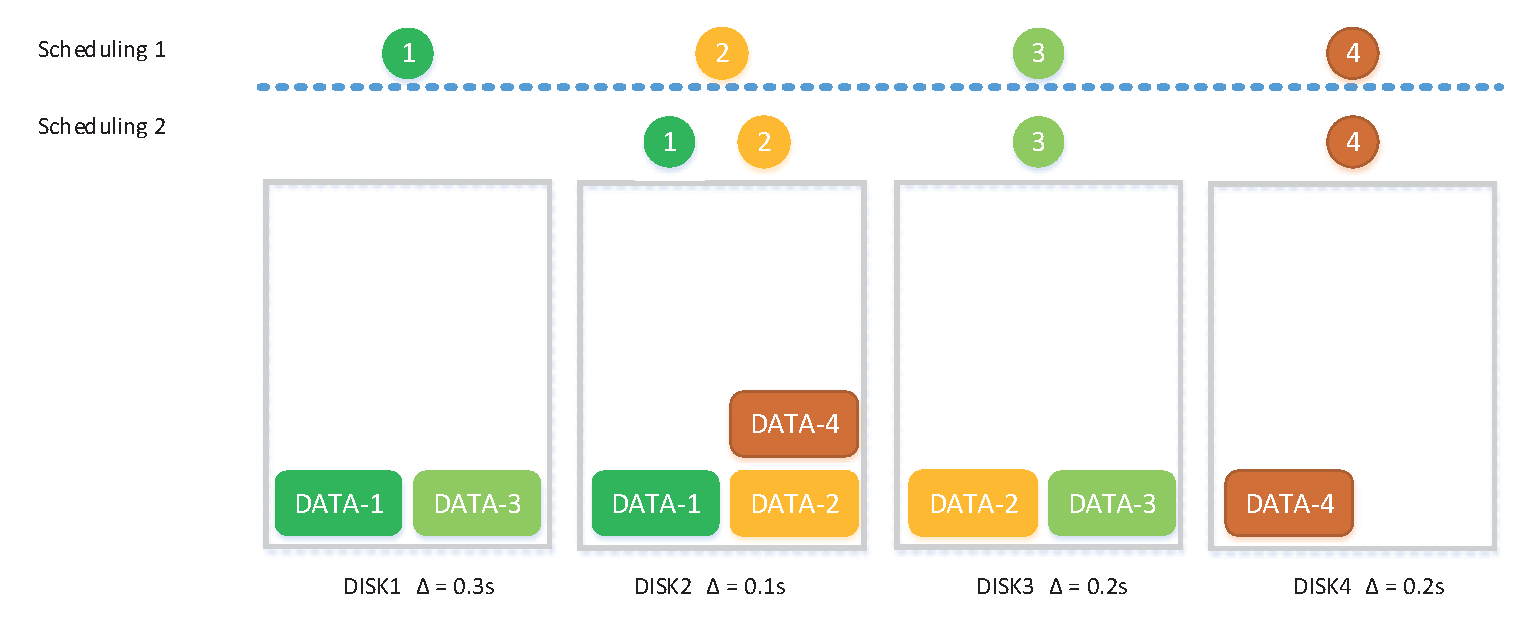
\includegraphics[height=0.8in]{fig2.eps}
	\caption{The process of algorithm HTS-greedy execution for the input in Fig.\ref{fig1}. }
	\label{fig2}
\end{figure}

The final result is in Result and  Tasks will follow \{$\left \langle t_1, d_{1}\right \rangle$, $\left \langle t_2, d_{2}\right \rangle$,  $\left \langle t_3, d_{3}\right \rangle$, $\left \langle t_4, d_{4}\right \rangle$\} to read data.The specific process of HTS-greedy algorithm is shown in Fig.\ref{fig2}.

\subsection{Randomized Alogrithm}\label{Randomized}

In the previous section \ref{Heuristic}, we designed a greedy heuristic algorithm HTS-greedy to solve HTS problems. However, this algorithm does not have a good performance guarantee. Therefore, in this section, we propose a performance-guaranteed random algorithm HTS-rdm. By relaxing the HTS problem to HTS-relaxation problem, HTS-rdm uses linear programming to solve HTS-relaxation. The decomposition obtained by linear programming is a fraction rather than an integer, which represents the preference when selecting disks. Subsequently, we prove that the solution found by the HTS-rdm algorithm can approach the optimal solution with a high probability.

\paragraph{\textbf{Relaxation of HTS Problem}} According to the previous analysis \ref{HTS}, this problem is NP-hard, which cannot be solved in polynomial time. Since the linear programming (LP) problem is solvable in polynomial time, a natural point of view is to relax the HTS problem to LP. The method is to change the range of variables from integer domain to real domain. As shown below, HTS-relaxtion, this process is named \textbf{relaxation}. The solution of HTS-relaxtion provides a lower bound for the original HTS problem(HTS is a minimization problem. For the maximization problem is on the contrary). Next, based on the solution of linear programming, the fractional solution is mapped back to integer in some way, which is named \textbf{rounding}. Based on relaxation-rounding, we propose HTS-rdm algorithm.

 \begin{align}
 Min:&\;\;\;\;\;\max\limits_{i}\{\sum_{j}p_i^j*T_i\}\;[\rm{HTS-relaxtion}]\nonumber\\
 s.t. 
 &\;\;\;\;\;\sum_{i}p_i^j = 1,\;for\;\forall j\nonumber\\
 &\;\;\;\;\;p_i^j \leq \pi_{\phi(t_j)}^{d_i},\;for\;\forall i,j\nonumber\\
 &\;\;\;\;\;p_i^j \in[0, 1],\;for\;\forall i,j\nonumber
 \end{align}
 
 The detailed procedure of HTS-rdm algorithm is shown in Algorithm\ref{HTS-rdm}. Line 1 initializes the Result set, which stores the final result. In the second line, the HTS-relaxation problem is solved by linear programming technique. The third line uses rounding strategy to convert fractional solution to integer solution. Line 4-9 organize the results and output them. Then the task will read the disk according to the Result. The specific rounding strategies are as follows:
 
 The value of \{$p_i^j$\}  $\in$ [0, 1] which shows the correlation between task $t_j$ and disk $d_i$. Therefore, we can select disk $d_i$ for task $t_j$ with  probability \{$p_i^j$\}. The method is to use the parameter $q_j$, which is randomly selected in (0,1]. If the $q_j$ $\in$ ($\sum p_{r-1}^{j}$, $\sum p_{r}^{j}$], then $I_r^j = 1$, otherwise, $I_i^j$ = 0 ($\forall$ $i$, $i \ne r$). This approach ensures only one disk can be selected for each task.%For each task $t_j$, the corresponding decision variables are \{$p_0^j$,$p_i^j$, ..., $p_i^j$\}. 
 \begin{algorithm}
 	%\renewcommand{\thealgorithm}{}
 	
 	\textbf{Require:} Decide a disk $d_i$ for each task $t_j$. %and $d_i$ stores data $\phi(t_j)$.
 	\begin{algorithmic}[1]
 		
 		\State Result $\gets$ \{\}
 		\State \{$p_i^j$\} = HTS-relaxtion		
 		$//$ is the solution of HTS-relaxtion problem. 
 		
 		\State Based on \{$p_i^j$\}, use rounding strategy and get \{$I_i^j$\}
 		\For{$\forall$ $i$, $j$}  
 			\If{$I_i^j$ == 1}
 			\State Result $\gets$ Result $\cup$ 	
 			\{$\left \langle t_j, d_i\right \rangle$\}
 			\EndIf
 		\EndFor	
 		\State \textbf{Return} Result	
 	\end{algorithmic}
 	\caption{HTS-rdm}\label{HTS-rdm}
 \end{algorithm}

\paragraph{\textbf{Analysis of HTS-rdm Algorithm}}

In this section, we will prove that the HTS-rdm algorithm can approach the optimal solution with a high probability. Firstly, we prove that the difference between $read-time$ contributed by any tasks $t_j$ to $d_i$ and expectation is matingales sequence \cite{b12}. Secondly, Based on the matigales sequence, we use Azuma inequality to illustrate the bound between the feasible solution and the optimal solution.
\begin{figure*}[!t]
	\centering
	\subfigure[Small-scale ]{\label{Fig:instance1}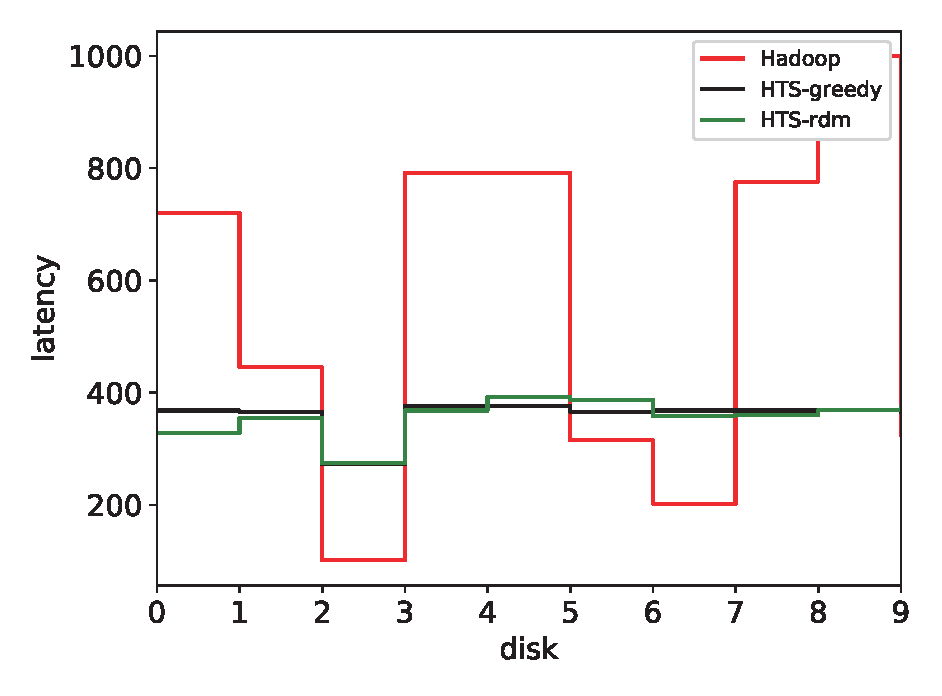
\includegraphics[height=1.6in]{fig3_1.eps}}\quad\quad %quad 表示图像的间距
	\subfigure[Medium-scale ]{\label{Fig:instance2}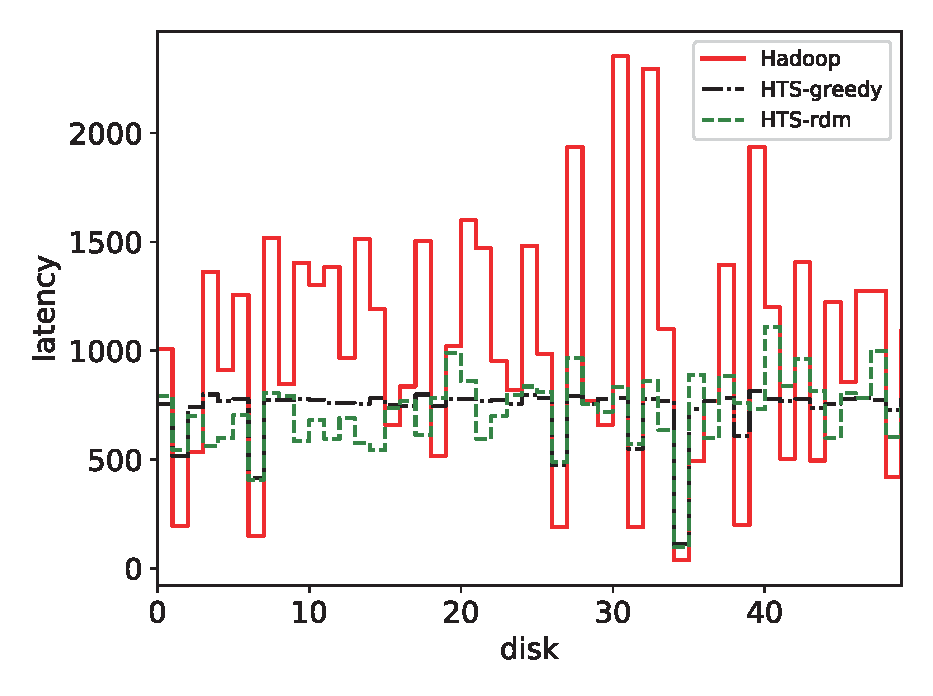
\includegraphics[height=1.6in]{fig3_2.eps}}\quad\quad
	\subfigure[Large-scale
	]{\label{Fig:instance3}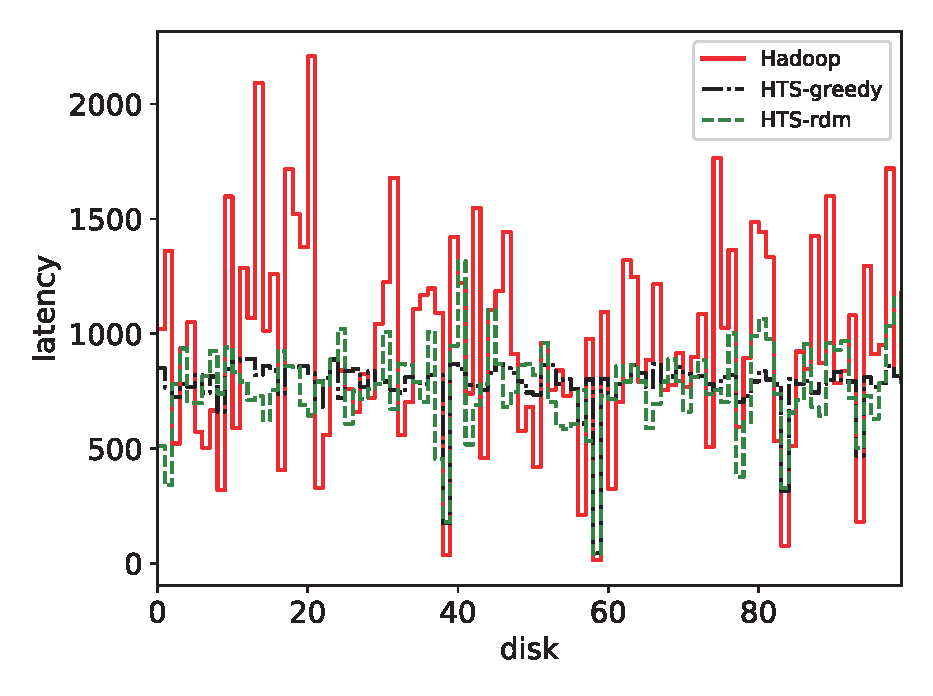
\includegraphics[height=1.6in]{fig3_4.eps}}
	\vspace{-2ex}
	\caption{Comparison of HTS-rdm and other Algorithm on different load. \ref{Fig:instance1} denotes Small-scale which has 20 task and 10 disks. \ref{Fig:instance2} denotes Medium-scale which has 200 task and 50 disks.
	\ref{Fig:instance3} denotes Large-scale which has 1000 task and 100 disks. X-axis denotes the disk id. Y-axis denotes the total $read-time$ of each disk after deploying the tasks.}
	\label{Fig:comparison}
	\vspace{-3ex}
\end{figure*}
\emph{Theorem 2:} Pr[SOL(HTS-rdm) - OPT(HTS) $\leq$ t] $\geq$ 1 - O($e^{-t^2}$).

\emph{Proof:}

SOL(HTS-rdm) means the solution found by HTS-rdm algorithm and  OPT(HTS) denotes the optimum solution of HTS problem.

Firstly, task $t_j$'s contribution to disk $d_i$'s $read-time$ is expressed as:
 \begin{align}
&\;\;\;\;\;Z_i^j = I_i^j*T_i
\end{align}

From the rounding strategy in Algorithm \ref{HTS-rdm}, we can get that:
 \begin{align}
&\;\;\;\;\;Pr[I_i^j = 1] = p_i^j,\;\;for\forall i,j \nonumber
\end{align}
%Therefore

The expectation of $Z_i^j$ is
\begin{align}
E[Z_i^j] &\;\;\;= E[I_i^j]*T_i \nonumber\\
&\;\;\;= (Pr[I_i^j = 1] * 1 + Pr[I_i^j = 0] * 0)*T_i \nonumber\\
&\;\;\;= p_i^j*T_i\label{prove:expect}
\end{align}

The difference between $Z_i^j$ and $E[Z_i^j]$ defines as
\begin{align}
Q_i^j = Z_i^j - E[Z_i^j]\label{prove:diff}
\end{align}

For the all $\mathbb{|T|}$ tasks, $L_i^{\mathbb{|T|}}$ denotes the sum of $Q_i^j$ in disk $d_i$:
\begin{align}
L_i^{\mathbb{|T|}} = \sum_{j = 1}^{\mathbb{|T|}} Q_i^j
= \sum_{j = 1}^{\mathbb{|T|} - 1} L_i^j + Q_i^{\mathbb{|T|}} \label{prove:L_margin}
\end{align}
Then, on the condition $L_i^{1}$, $L_i^{2}$, ..., $L_i^{r-1}$, the expectation of $L_i^{r}$ is:
\begin{align}
&E[L_i^{r}|L_i^{1}, L_i^{2}, ..., L_i^{r-1}] \nonumber\\
&\overset{\text{(\ref{prove:L_margin})}}{=}E[L_i^{r-1} + Q_i^{r} |L_i^{1}, L_i^{2}, ..., L_i^{r-1}] \nonumber\\
&\overset{\text{}}{=}E[L_i^{r-1} |L_i^{1}, L_i^{2}, ..., L_i^{r-1}]
+ E[Q_i^{r} |L_i^{1}, L_i^{2}, ..., L_i^{r-1}] \nonumber\\
&\overset{\text{(\ref{prove:diff})}}{=}L_i^{r-1} + E[Z_i^r - E[Z_i^r] |L_i^{1}, L_i^{2}, ..., L_i^{r-1}]\nonumber\\
&=L_i^{r-1} + E[Z_i^r|L_i^{1}, L_i^{2}, ..., L_i^{r-1}]
-E[E[Z_i^r] |L_i^{1}, L_i^{2}, ..., L_i^{r-1}]\nonumber\\
&=L_i^{r-1} + E[Z_i^r] - E[Z_i^r]\nonumber\\
&=L_i^{r-1}\label{prove:marginsq}
\end{align}
Therefore, $L_i^{1}$, $L_i^{2}$, ..., $L_i^{|\mathbb{T}|}$ are matigales sequence \cite{b13}. For completeness, we let $L_i^{0}$ = 0. And for $\forall r \geq 1$, we have:
\begin{align}
  |L_i^r - L_i^{r-1}|\overset{\text{(\ref{prove:L_margin})}}{=} |Q_i^{r}| \overset{\text{(\ref{prove:diff})}}{=} |Z_i^j - E[Z_i^j]|\leq g_i^r\\
  g_i^r = \max\{T_i -  E[Z_i^j], E[Z_i^j]\}\label{prove:bound}
\end{align}

From above (\ref{prove:bound}), any two adjacent values $L_i^r$, $L_i^{r-1}$ in the margingales sequence have constant bounds $g_i^r$. Based on (\ref{prove:marginsq}) and (\ref{prove:bound}), we can use Azuma's inequality. Then, 

\begin{align}
Pr\{L_i^{|\mathbb{T}|} - L_i^{0} \geq t\} \leq exp\{-\frac{t^2}{2\sum_{ i = 1 }^{|\mathbb{T}|}(g_i^k)^2}\} \label{prove:azuma}
\end{align}

Substitute equations (\ref{prove:diff}) and (\ref{prove:L_margin}) into the upper equation (\ref{prove:azuma}). Then, 

\begin{align}
Pr\{\sum_{j = 1}^{|\mathbb{T}|} Z_i^j - 
	\sum_{j = 1}^{|\mathbb{T}|} E[Z_i^j]\geq t\} \leq exp\{-\frac{t^2}{2\sum_{ i = 1 }^{|\mathbb{T}|}(g_i^k)^2}\} \label{prove:azuma1}
\end{align}
 The (\ref{prove:azuma1}) is equal to:
\begin{align}
Pr\{\sum_{j = 1}^{|\mathbb{T}|} Z_i^j \leq \sum_{j = 1}^{|\mathbb{T}|} E[Z_i^j] + t\} \geq 1 - exp\{-\frac{t^2}{2\sum_{ i = 1 }^{|\mathbb{T}|}(g_i^k)^2}\}\nonumber\\
= 1 - O(e^{-t^2})\label{prove:azuma3}
\end{align}

Let $S_i$  = $\sum_{j = 1}^{|\mathbb{T}|} Z_i^j$,
$E_i$ = $\sum_{j = 1}^{|\mathbb{T}|} E[Z_i^j]$
$\overset{\text{(\ref{prove:expect})}}{=}$
$\sum_{j = 1}^{|\mathbb{T}|} p_i^j*T_i$. Then,
\begin{align}
Pr\{S_i \leq U_i + t\} \geq 1- O(e^{-t^2}) \label{prove:SU}
\end{align}

$S_i$ denotes the total $read-time$ of disk $d_i$ which is the result of ILP. And $E_i$ denotes the expectation which is the result of LP. Because LP provides a lower bound for the optimal solution of ILP problem (HTS is a minimization problem. For the maximization problem is on the contrary), we have:



\begin{align}
E_i \leq OPT(HTS)\label{prove:OPT}
\end{align}

Take $S_u$, $E_v$ as
\begin{align}
	S_u = S_{max} = \max_i S_i\\
	E_v = E_{max} = \max_i E_i\label{prove:Emax}
\end{align}

Then, we have the following inequalities,
\begin{align}
SOL(HTS-rdm) = S_u  
\overset{\text{(\ref{prove:azuma3})}}{\leq}  E_u+t
\overset{\text{(\ref{prove:Emax})}}{\leq} E_v+t\nonumber\\
\overset{\text{(\ref{prove:OPT})}}{\leq} OPT(HTS)+t\label{prove:SOL-OPT}
\end{align}

From (\ref{prove:SU}) and (\ref{prove:SOL-OPT}), we can conclude that,
\begin{align}
Pr\{SOL(HTS-rdm)<OPT (HTS)+t\} \geq 1 - O(e^{-t^2})\label{prove:result}
\end{align}

Observed from the (\ref{prove:result}), the feasible solution SOL(HTS-rdm) found by the algorithm and the optimal solution OPT (HTS) are approximated by probability $1 - O(e^{-t^2})$. When hundreds of tasks are deployed with $1 - O(e^{-t^2})$ = 0.85, the value of $t$ is acceptable, only a few millisecond.\hfill $\qedsymbol$


fdd
\section{PERFORMANCE EVALUATION}\label{PERFORMANCE_EVALUATION}
\subsection{Simulation Settings}\label{SCM}

\subsection{Simulation Results}

%
%\begin{figure}
%	\centering
%	\includegraphics[height=2in]{instance333.eps}
%	\vspace{-2ex}
%	\caption{An execution instace of the three algorithm}
%\end{figure}







\section{CONCLUSION}\label{CONCLUSION}
None

\section*{Acknowledgment}

None





\begin{thebibliography}{00}
\bibitem{b1} Ahmad F, Chakradhar S T, Raghunathan A, et al. Tarazu: optimizing mapreduce on heterogeneous clusters[C]//ACM SIGARCH Computer Architecture News. ACM, 2012, 40(1): 61-74.
\bibitem{b2} Zaharia M, Borthakur D, Sen Sarma J, et al. Delay scheduling: a simple technique for achieving locality and fairness in cluster scheduling[C]//Proceedings of the 5th European conference on Computer systems. ACM, 2010: 265-278.
\bibitem{b3} Ananthanarayanan G, Agarwal S, Kandula S, et al. Scarlett: coping with skewed content popularity in mapreduce clusters[C]//Proceedings of the sixth conference on Computer systems. ACM, 2011: 287-300.
\bibitem{b4} Abad C L, Lu Y, Campbell R H. DARE: Adaptive data replication for efficient cluster scheduling[C]//2011 IEEE international conference on cluster computing. IEEE, 2011: 159-168.
\bibitem{b5} Jalaparti V, Bodik P, Menache I, et al. Network-aware scheduling for data-parallel jobs: Plan when you can[C]//ACM SIGCOMM Computer Communication Review. ACM, 2015, 45(4): 407-420.
\bibitem{b6} Xu L, Butt A R, Lim S H, et al. A heterogeneity-aware task scheduler for spark[C]//2018 IEEE International Conference on Cluster Computing (CLUSTER). IEEE, 2018: 245-256.
\bibitem{b7} Pan F, Xiong J, Shen Y, et al. H-Scheduler: Storage-Aware Task Scheduling for Heterogeneous-Storage Spark Clusters[C]//2018 IEEE 24th International Conference on Parallel and Distributed Systems (ICPADS). IEEE, 2018: 1-9.
\bibitem{b8} Wang B, Jiang J, Yang G. Actcap: Accelerating mapreduce on heterogeneous clusters with capability-aware data placement[C]//2015 IEEE Conference on Computer Communications (INFOCOM). IEEE, 2015: 1328-1336.
\bibitem{b9} Karp R M. Reducibility among combinatorial problems[M]//Complexity of computer computations. Springer, Boston, MA, 1972: 85-103.
\bibitem{b10} Hromkovič J. Algorithmics for hard problems: introduction to combinatorial optimization, randomization, approximation, and heuristics[M]. Springer Science \& Business Media, 2013.
\bibitem{b11} 2018. Integer programming. https://en.wikipedia.org/wiki/Integer\_programming.
\bibitem{b12} Grimmett G, Grimmett G R, Stirzaker D. Probability and random processes[M]. Oxford university press, 2001.
\bibitem{b13} 2019. Martingale (probability theory). https://en.wikipedia.org/wiki/Martingale\_(probability\_theory)

\bibitem{b14} Wang B, Jiang J, Yang G. Actcap: Accelerating mapreduce on heterogeneous clusters with capability-aware data placement[C]//2015 IEEE Conference on Computer Communications (INFOCOM). IEEE, 2015: 1328-1336.
\bibitem{b15} Apache Spark. https://spark.apache.org, 2019.
\bibitem{b16}Dell. https://www.dell.com/zh-cn,2019.
\bibitem{b17}Samsung. https://www.samsung.com/semiconductor/cn/, 2019.
\bibitem{b18}Guo Z, Fox G, Zhou M. Investigation of data locality in mapreduce[C]//Proceedings of the 2012 12th IEEE/ACM International Symposium on Cluster, Cloud and Grid Computing (ccgrid 2012). IEEE Computer Society, 2012: 419-426.
\bibitem{b19} Hdfs. https://hadoop.apache.org/hdfs, 2019.

\end{thebibliography}
\end{document}

